\documentclass[12pt, letterpaper]{article}
  \usepackage[utf8]{inputenc}
  \usepackage[left = 2.5cm, right = 2.5cm, top = 3cm, bottom = 3cm]{geometry}
  \usepackage[T1]{fontenc}
  \usepackage{graphicx}
  \usepackage{tikz}
  \usetikzlibrary{automata,positioning}
  \graphicspath{{images/}}

  \author{Hernández Ferreiro Enrique Ehécatl \\
          López Soto Ramses Antonio}

        \title{Práctica 5: Lógica Secuencial \\
                {\small Organización y Arquitectura de Computadoras}}
                \date{13 de marzo de 2019}

  \begin{document}
    \maketitle

    \section{Introducción}

      \hspace{.5cm}
      Los circuitos que ya hemos visto han sido lógicos, es decir, sólo dependen
      de sus entradas, pero en la mayoría de los casos las computadoras incluyen
      dispositivos de almacenamiento, por lo que la construcción de los circuitos
      deben ser en términos secuenciales.\vspace{.3cm}

      Un circuito secuencial es aquel en el que sus salidas no sólo dependen de
      sus entradas, sino también de su posición y su estado actual, almacenada
      elementos de memoria.\vspace{.3cm}

      Los elementos de almacenamiento son dispositivos que almacenan la
      información en forma binaria, en la cual se define el estado del circuito,
      que se encarga de recibir la información de entradas externas, las cuales,
      junto con el estado que esta almacenadoe ne la memoria, se determina el
      de las salidas, asi como la condición, para ambiar de estado.

    \section{Desarrollo}
      \subsection*{Autómata}
        \begin{center}
          \begin{table}[htb]
            \begin{tabular}{lllllllll}
              A & B & In & A1 & B1 & Sa & Ra & Sb & Rb \\
              0 & 0 & 0  & 0  & 1  & 0  & X  & 1  & 0  \\
              0 & 0 & 1  & 0  & 0  & 0  & X  & 0  & X  \\
              0 & 1 & 0  & 1  & 0  & 1  & 0  & 0  & 1  \\
              0 & 1 & 1  & 0  & 0  & 0  & X  & 0  & 1  \\
              1 & 0 & 0  & 1  & 1  & X  & 0  & 1  & 0  \\
              1 & 0 & 1  & 1  & 0  & X  & 0  & 0  & X  \\
              1 & 1 & 0  & 0  & 0  & 0  & 1  & 0  & 1  \\
              1 & 1 & 1  & 0  & 0  & X  & 0  & 0  & 1
            \end{tabular}
            \caption{Tabla de verdad del autómata}
          \end{table}
        \end{center}

        \begin{center}
          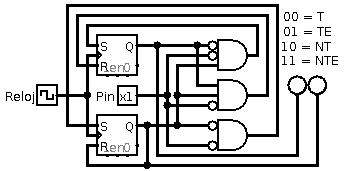
\includegraphics{automata.png}
        \end{center}


    \section{Conclusión}

      \subsection{Preguntas}

        \begin{itemize}
          \item[1.] ¿En qué difieren los distintos tios de flip-flop? ¿Cómo se
                    decide que tipo se usará en el circuito?
                    R. 
          \item[2.] Un \textbf{registro de desplazamiento} es un circuito
                    secuencial que desplaza a la izquierda o a la derecha la
                    información contenida en él. Considerando el desplazamiento
                    de 1 bit a la izquierda, ¿cómo se implementa dicho circuito?
                    ¿Cómo podríamos simular su funcionamiento con las operaciones
                    que se tienen en la ALU de 8 bits?
        \end{itemize}

  \end{document}
